\documentclass[10pt]{beamer}

% Configuración de idioma y codificación
\usepackage[utf8]{inputenc}
\usepackage[spanish]{babel}
\usepackage{amsmath}
\usepackage{amssymb}
\usepackage{hyperref}
\usepackage{graphicx}
\usepackage{listings}
\usepackage{xcolor}
\usepackage{booktabs}
\usepackage{tikz}

% -------------------------------------------------------------------
% CONFIGURACIÓN DE COLORES TIPO ICMAT
% -------------------------------------------------------------------
\usetheme{Madrid}

\definecolor{IcmatOrange}{HTML}{EC8810}
\definecolor{IcmatDarkGrey}{HTML}{2C2C2C}
\definecolor{CodeBg}{HTML}{1a1a2e}
\definecolor{CodeKw}{HTML}{e74c3c}
\definecolor{CodeStr}{HTML}{2ecc71}
\definecolor{CodeCmt}{HTML}{95a5a6}
\definecolor{CodeId}{HTML}{3498db}

\usecolortheme[named=IcmatOrange]{structure}
\setbeamercolor{palette primary}{bg=IcmatOrange,fg=white}
\setbeamercolor{palette secondary}{bg=IcmatDarkGrey,fg=white}
\setbeamercolor{palette tertiary}{bg=black,fg=white}
\setbeamercolor{frametitle}{bg=IcmatDarkGrey,fg=white}
\setbeamercolor{block title}{bg=IcmatOrange,fg=white}
\setbeamercolor{block body}{bg=IcmatDarkGrey!15}
\setbeamercolor{block title alerted}{bg=IcmatDarkGrey,fg=IcmatOrange}
\setbeamercolor{block body alerted}{bg=IcmatDarkGrey!10}

% Estilo de código Python
\lstdefinestyle{python}{
  language=Python,
  backgroundcolor=\color{CodeBg},
  basicstyle=\ttfamily\scriptsize\color{white},
  keywordstyle=\color{CodeKw}\bfseries,
  stringstyle=\color{CodeStr},
  commentstyle=\color{CodeCmt}\itshape,
  identifierstyle=\color{CodeId},
  numberstyle=\tiny\color{CodeCmt},
  breaklines=true,
  frame=none,
  xleftmargin=4pt,
  xrightmargin=4pt,
  aboveskip=4pt,
  belowskip=2pt,
}

% -------------------------------------------------------------------
% METADATOS
% -------------------------------------------------------------------
\title[Neural ODEs de Campo Medio — Make Moons]{Neural ODEs de Campo Medio\\con Regularización Entrópica}
\subtitle{Verificación empírica de arXiv:2507.08486\\(Daudin \& Delarue, 2025)}
\author[Daniel Torres]{Daniel Torres}
\institute[CSIC]{Consejo Superior de Investigaciones Científicas (CSIC)\\
Beca de Introducción a la Investigación JAE\\
\medskip
{\small Tutor: Rafael Orive}}
\date{\today}

\titlegraphic{\vspace{-0.75cm}\includegraphics[height=1.8cm]{logo_icmat.jpg}}

% -------------------------------------------------------------------
\begin{document}

\begin{frame}
  \titlepage
\end{frame}

% ===================================================================
\begin{frame}{Índice}
  \tableofcontents
\end{frame}

% ===================================================================
\section{Motivación y marco teórico}

\begin{frame}{Redes neuronales como sistemas de control}

\begin{columns}
\column{0.55\textwidth}
Una ResNet profunda con $L$ capas:
\[
  X_{k+1} = X_k + \frac{1}{L}\,F_k(X_k), \quad k=0,\ldots,L-1
\]
En el límite $L\to\infty$, con paso $dt = 1/L$, se obtiene la \textbf{Neural ODE}:
\[
  \frac{dX_t}{dt} = F(X_t, t), \quad t\in[0,T]
\]

En el límite $M\to\infty$ neuronas por capa, la distribución de parámetros converge a una \textbf{medida de control}:
\[
  F(x,t) = \int_A b(x,a)\,d\nu_t(a)
\]
\column{0.42\textwidth}
\begin{block}{Dos límites simultáneos}
  \begin{tabular}{ll}
    \toprule
    Límite & Resultado \\
    \midrule
    $L\to\infty$ & Neural ODE \\
    $M\to\infty$ & Campo medio \\
    \bottomrule
  \end{tabular}
  \medskip\\
  El problema se convierte en \textbf{optimizar sobre trayectorias de medidas} $(\nu_t)_{t\in[0,T]}$, no sobre vectores de parámetros $\theta\in\mathbb{R}^p$.
\end{block}
\end{columns}

\bigskip
\begin{alertblock}{Referencia}
  Daudin, S.\ \& Delarue, F.\ (2025). \textit{Genericity of the Polyak-Łojasiewicz inequality for mean-field Neural ODEs with entropic regularization.} arXiv:2507.08486
\end{alertblock}
\end{frame}

% -------------------------------------------------------------------
\begin{frame}{Campo vectorial prototípico}

\begin{block}{Campo vectorial (Ejemplo 1.1, ec.\ 1.8 del paper)}
\[
  b(x,a) = \sigma\!\left(a_1 \cdot x + a_2\right)\cdot a_0, \qquad \sigma = \tanh
\]
donde $a = (a_0, a_1, a_2)\in A = \mathbb{R}^{d_1}\times\mathbb{R}^{d_1}\times\mathbb{R}$.
\end{block}

\bigskip
Con $M$ partículas (aproximación de $\nu_t$ por $M$ muestras discretas):
\[
  F(x,t) \approx \frac{1}{M}\sum_{m=1}^{M} \sigma\!\left(a_1^m\cdot x + a_2^m\right)\cdot a_0^m
\]

\medskip
Esto es exactamente una \textbf{red de una capa oculta con $M$ neuronas}.

\bigskip
\begin{columns}
\column{0.48\textwidth}
\begin{block}{Activación $\tanh$}
  Satisface la propiedad discriminante (sec.\ 1.2): el campo $b(x,\cdot)$ puede aproximar cualquier función continua.
\end{block}
\column{0.48\textwidth}
\begin{block}{Distribución de parámetros}
  En el límite de campo medio: $\nu_t\in\mathcal{P}(A)$ en lugar de $M$ parámetros discretos.
\end{block}
\end{columns}
\end{frame}

% -------------------------------------------------------------------
\begin{frame}{Ecuación de continuidad y distribución de datos}

La distribución conjunta $\gamma_t\in\mathcal{P}(\mathbb{R}^{d_1}\times\mathbb{R}^{d_2})$ evoluciona según:
\[
  \partial_t\gamma_t + \operatorname{div}_x\!\bigl(F(x,t)\,\gamma_t\bigr) = 0
\]

\begin{columns}
\column{0.52\textwidth}
\begin{itemize}
  \item $\gamma_t$ es la distribución \textbf{conjunta} (features + etiquetas)
  \item La ODE mueve solo $x\in\mathbb{R}^{d_1}$; la etiqueta $y\in\mathbb{R}^{d_2}$ se transporta pasivamente
  \item El flujo es $\phi_t(x_0,y) = (X_t,\,y)$
\end{itemize}

\medskip
La solución formal:
\[
  \gamma_t = (\phi_t)_\sharp\,\gamma_0
\]

\column{0.44\textwidth}
\begin{alertblock}{Notación (Make Moons)}
  \begin{align*}
    d_1 &= 2 \text{ (features $\in\mathbb{R}^2$)}\\
    d_2 &= 1 \text{ (etiqueta $\in\mathbb{R}$)}\\[4pt]
    \gamma_0 &= \frac{1}{N}\sum_i\delta_{(X_0^i,Y_0^i)}\\[4pt]
    \gamma_t &= \frac{1}{N}\sum_i\delta_{(X_t^i,Y_0^i)}
  \end{align*}
  Las figuras muestran la \textbf{marginal en $x$} de $\gamma_t$.
\end{alertblock}
\end{columns}
\end{frame}

% -------------------------------------------------------------------
\begin{frame}{Regularización entrópica y función objetivo}

\begin{block}{Función objetivo del control (ec.\ 1.6)}
\[
  J(\gamma_0,\nu) = \underbrace{\int L(x,y)\,d\gamma_T(x,y)}_{\text{coste terminal (BCE)}} + \underbrace{\varepsilon\int_0^T \mathcal{E}(\nu_t\mid\nu^\infty)\,dt}_{\text{penalización entrópica}}
\]
\end{block}

\medskip
El prior es $\nu^\infty(da)\propto e^{-\ell(a)}\,da$ con potencial \textbf{supercoercivo}:
\[
  \ell(a) = c_1|a|^4 + c_2|a|^2, \qquad c_1 = 0.05,\quad c_2 = 0.5
\]

\begin{columns}
\column{0.48\textwidth}
\begin{block}{Control óptimo (ec.\ 1.9)}
  \[
    \nu_t^*(da) \propto \exp\!\!\left(-\ell(a) - \tfrac{1}{\varepsilon}\int b(x,a)\cdot\nabla u_t\,d\gamma_t\right)da
  \]
  Forma de \textbf{Gibbs}: concentra $\nu_t^*$ en los parámetros que minimizan $L$ penalizados por $\ell(a)$.
\end{block}
\column{0.48\textwidth}
\begin{block}{Por qué $c_1 > 0$ es esencial}
  El crecimiento cuártico garantiza la \textbf{desigualdad log-Sobolev}:
  \[
    \mathcal{E}(\mu\mid\nu^\infty) \leq \frac{1}{2\rho}\,\mathcal{I}(\mu\mid\nu^\infty)
  \]
  que implica la condición PL.
\end{block}
\end{columns}
\end{frame}

% -------------------------------------------------------------------
\begin{frame}{Los dos Meta-Teoremas}

\begin{block}{Meta-Teorema 1 — Genericidad (sec.\ 1.3)}
  Existe un conjunto \textbf{abierto y denso} $\mathcal{O}\subset\mathcal{P}(\mathbb{R}^{d_1}\times\mathbb{R}^{d_2})$ tal que para todo $\gamma_0\in\mathcal{O}$, el problema de control tiene un \textbf{único minimizador estable}.
  \medskip\\
  \textit{«Casi toda distribución inicial de datos produce un paisaje de pérdida con un único mínimo profundo.»}
\end{block}

\bigskip
\begin{block}{Meta-Teorema 2 — Condición PL local (sec.\ 1.4)}
  Para $\gamma_0\in\mathcal{O}$ y $\varepsilon > 0$, la \textbf{desigualdad de Polyak-Łojasiewicz} se cumple localmente:
  \[
    \|\nabla J(\theta)\|^2 \;\geq\; 2\mu\cdot(J(\theta)-J^*)
  \]
  con $\mu > 0$ dependiente de $\varepsilon$ (pero no necesita ser grande).\\[4pt]
  \textbf{Corolario:} convergencia \textbf{exponencial} sin convexidad:
  \[
    J(\theta_k) - J^* \;\leq\; (1-2\eta\mu)^k \cdot (J(\theta_0)-J^*)
  \]
\end{block}

\end{frame}

% ===================================================================
\section{Implementación}

\begin{frame}[fragile]{Dataset: Make Moons}

\begin{columns}
\column{0.52\textwidth}
\begin{lstlisting}[style=python]
def get_moons(n=400, noise=0.12, seed=SEED):
    # gamma_0 = (1/N) sum delta_{(X0i, Y0i)}
    # en R^{d1} x R^{d2} = R^2 x R
    X_np, y_np = make_moons(
        n_samples=n, noise=noise,
        random_state=seed)
    X_np = StandardScaler()\
               .fit_transform(X_np)\
               .astype(np.float32)
    y_np = y_np.astype(np.float32)
    return (torch.tensor(X_np, device=DEVICE),
            torch.tensor(y_np, device=DEVICE),
            X_np, y_np)
\end{lstlisting}

\column{0.44\textwidth}
\begin{block}{Parámetros}
  \begin{tabular}{ll}
    $N$ & 400 puntos \\
    $\sigma$ & 0.12 (ruido) \\
    $d_1$ & 2 (features) \\
    $d_2$ & 1 (etiqueta) \\
  \end{tabular}
\end{block}
\medskip
$\gamma_0$ es \textbf{no separable linealmente}: las dos clases forman medias lunas entrelazadas.
\medskip\\
\[
  \gamma_0 = \frac{1}{N}\sum_{i=1}^N\delta_{(X_0^i,Y_0^i)}
\]
\end{columns}
\end{frame}

% -------------------------------------------------------------------
\begin{frame}[fragile]{Arquitectura: MeanFieldResNet}

\[
  X_0\in\mathbb{R}^2 \;\xrightarrow{\text{ODE, }t\in[0,1]}\; X_T\in\mathbb{R}^2 \;\xrightarrow{W,b}\; \text{logit}\in\mathbb{R}
\]

\begin{columns}
\column{0.52\textwidth}
\begin{lstlisting}[style=python]
class MeanFieldVelocity(nn.Module):
    # Implementa b(x,a) = sigma(a1*x+a2)*a0
    # con time-augmentation: [x, t] como input
    def forward(self, x, t):
        # x: (N, d1),  t: escalar
        t_col = t * torch.ones(
            x.shape[0], 1, device=x.device)
        xt = torch.cat([x, t_col], dim=1)
        # h = tanh(W1 [x,t]^T + b1), shape (N,M)
        h = torch.tanh(
            xt @ self.W1.T + self.b1)
        # F(x,t) = h W0^T / M, shape (N, d1)
        return h @ self.W0.T / self.M
\end{lstlisting}
\column{0.44\textwidth}
\begin{block}{Parámetros del modelo}
  \begin{tabular}{ll}
    $M$ & 64 neuronas \\
    $T$ & 1.0 \\
    \texttt{n\_steps} & 10 (RK4) \\
    $\approx$ & 450 parámetros \\
  \end{tabular}
\end{block}
\medskip
\begin{alertblock}{Aproximación: augmentación temporal}
  Los pesos $(W_0,W_1,b_1)$ son \textbf{estáticos}; $t$ se concatena como feature adicional. Restringe $\nu_t$ a una familia paramétrica concreta (menor que el espacio completo del paper).
\end{alertblock}
\end{columns}
\end{frame}

% -------------------------------------------------------------------
\begin{frame}[fragile]{Integrador RK4 y función objetivo}

\begin{columns}
\column{0.50\textwidth}
\begin{lstlisting}[style=python]
def _rk4(self, x, t, dt):
    # Error local O(dt^5); global O(dt^4)
    k1 = self.vel(x, t)
    k2 = self.vel(x + dt/2*k1, t + dt/2)
    k3 = self.vel(x + dt/2*k2, t + dt/2)
    k4 = self.vel(x + dt*k3,   t + dt)
    return x + dt/6*(k1+2*k2+2*k3+k4)
\end{lstlisting}

\medskip
\begin{tabular}{lll}
\toprule
Método & Error local & Error global \\
\midrule
Euler & $O(dt^2)$ & $O(dt) \approx 0.1$ \\
RK4   & $O(dt^5)$ & $O(dt^4)\approx 10^{-4}$ \\
\bottomrule
\end{tabular}

\column{0.47\textwidth}
\begin{block}{Función objetivo implementada}
\[
  J(\theta) = \underbrace{\frac{1}{N}\sum_i\mathrm{BCE}_i}_{\text{coste terminal}} + \varepsilon\cdot\underbrace{\frac{1}{N_\theta}\sum_j\bigl[c_1\theta_j^4 + c_2\theta_j^2\bigr]}_{\text{energía de }\mathcal{E}(\nu\mid\nu^\infty)}
\]
\end{block}
\begin{alertblock}{Aproximación: término entrópico}
  Solo se usa el \textbf{término de energía} $\mathbb{E}_{\nu_t}[\ell(a)]$. La entropía $H(\nu_t)=-\infty$ para medidas discretas (parámetros deterministas). Equivale a regularización L4+L2.
\end{alertblock}
\end{columns}
\end{frame}

% ===================================================================
\section{Experimento A — Evolución de $\gamma_t$}

\begin{frame}{Experimento A — Evolución de $\gamma_t$}

\textbf{Objetivo:} visualizar cómo la ODE transforma $\gamma_0$ (lunas entrelazadas) en $\gamma_T$ (clases separables), verificando la ecuación de continuidad.

\medskip
Configuración: $\varepsilon = 0.01$, $M = 64$, $T = 1.0$, 800 épocas.

\begin{center}
  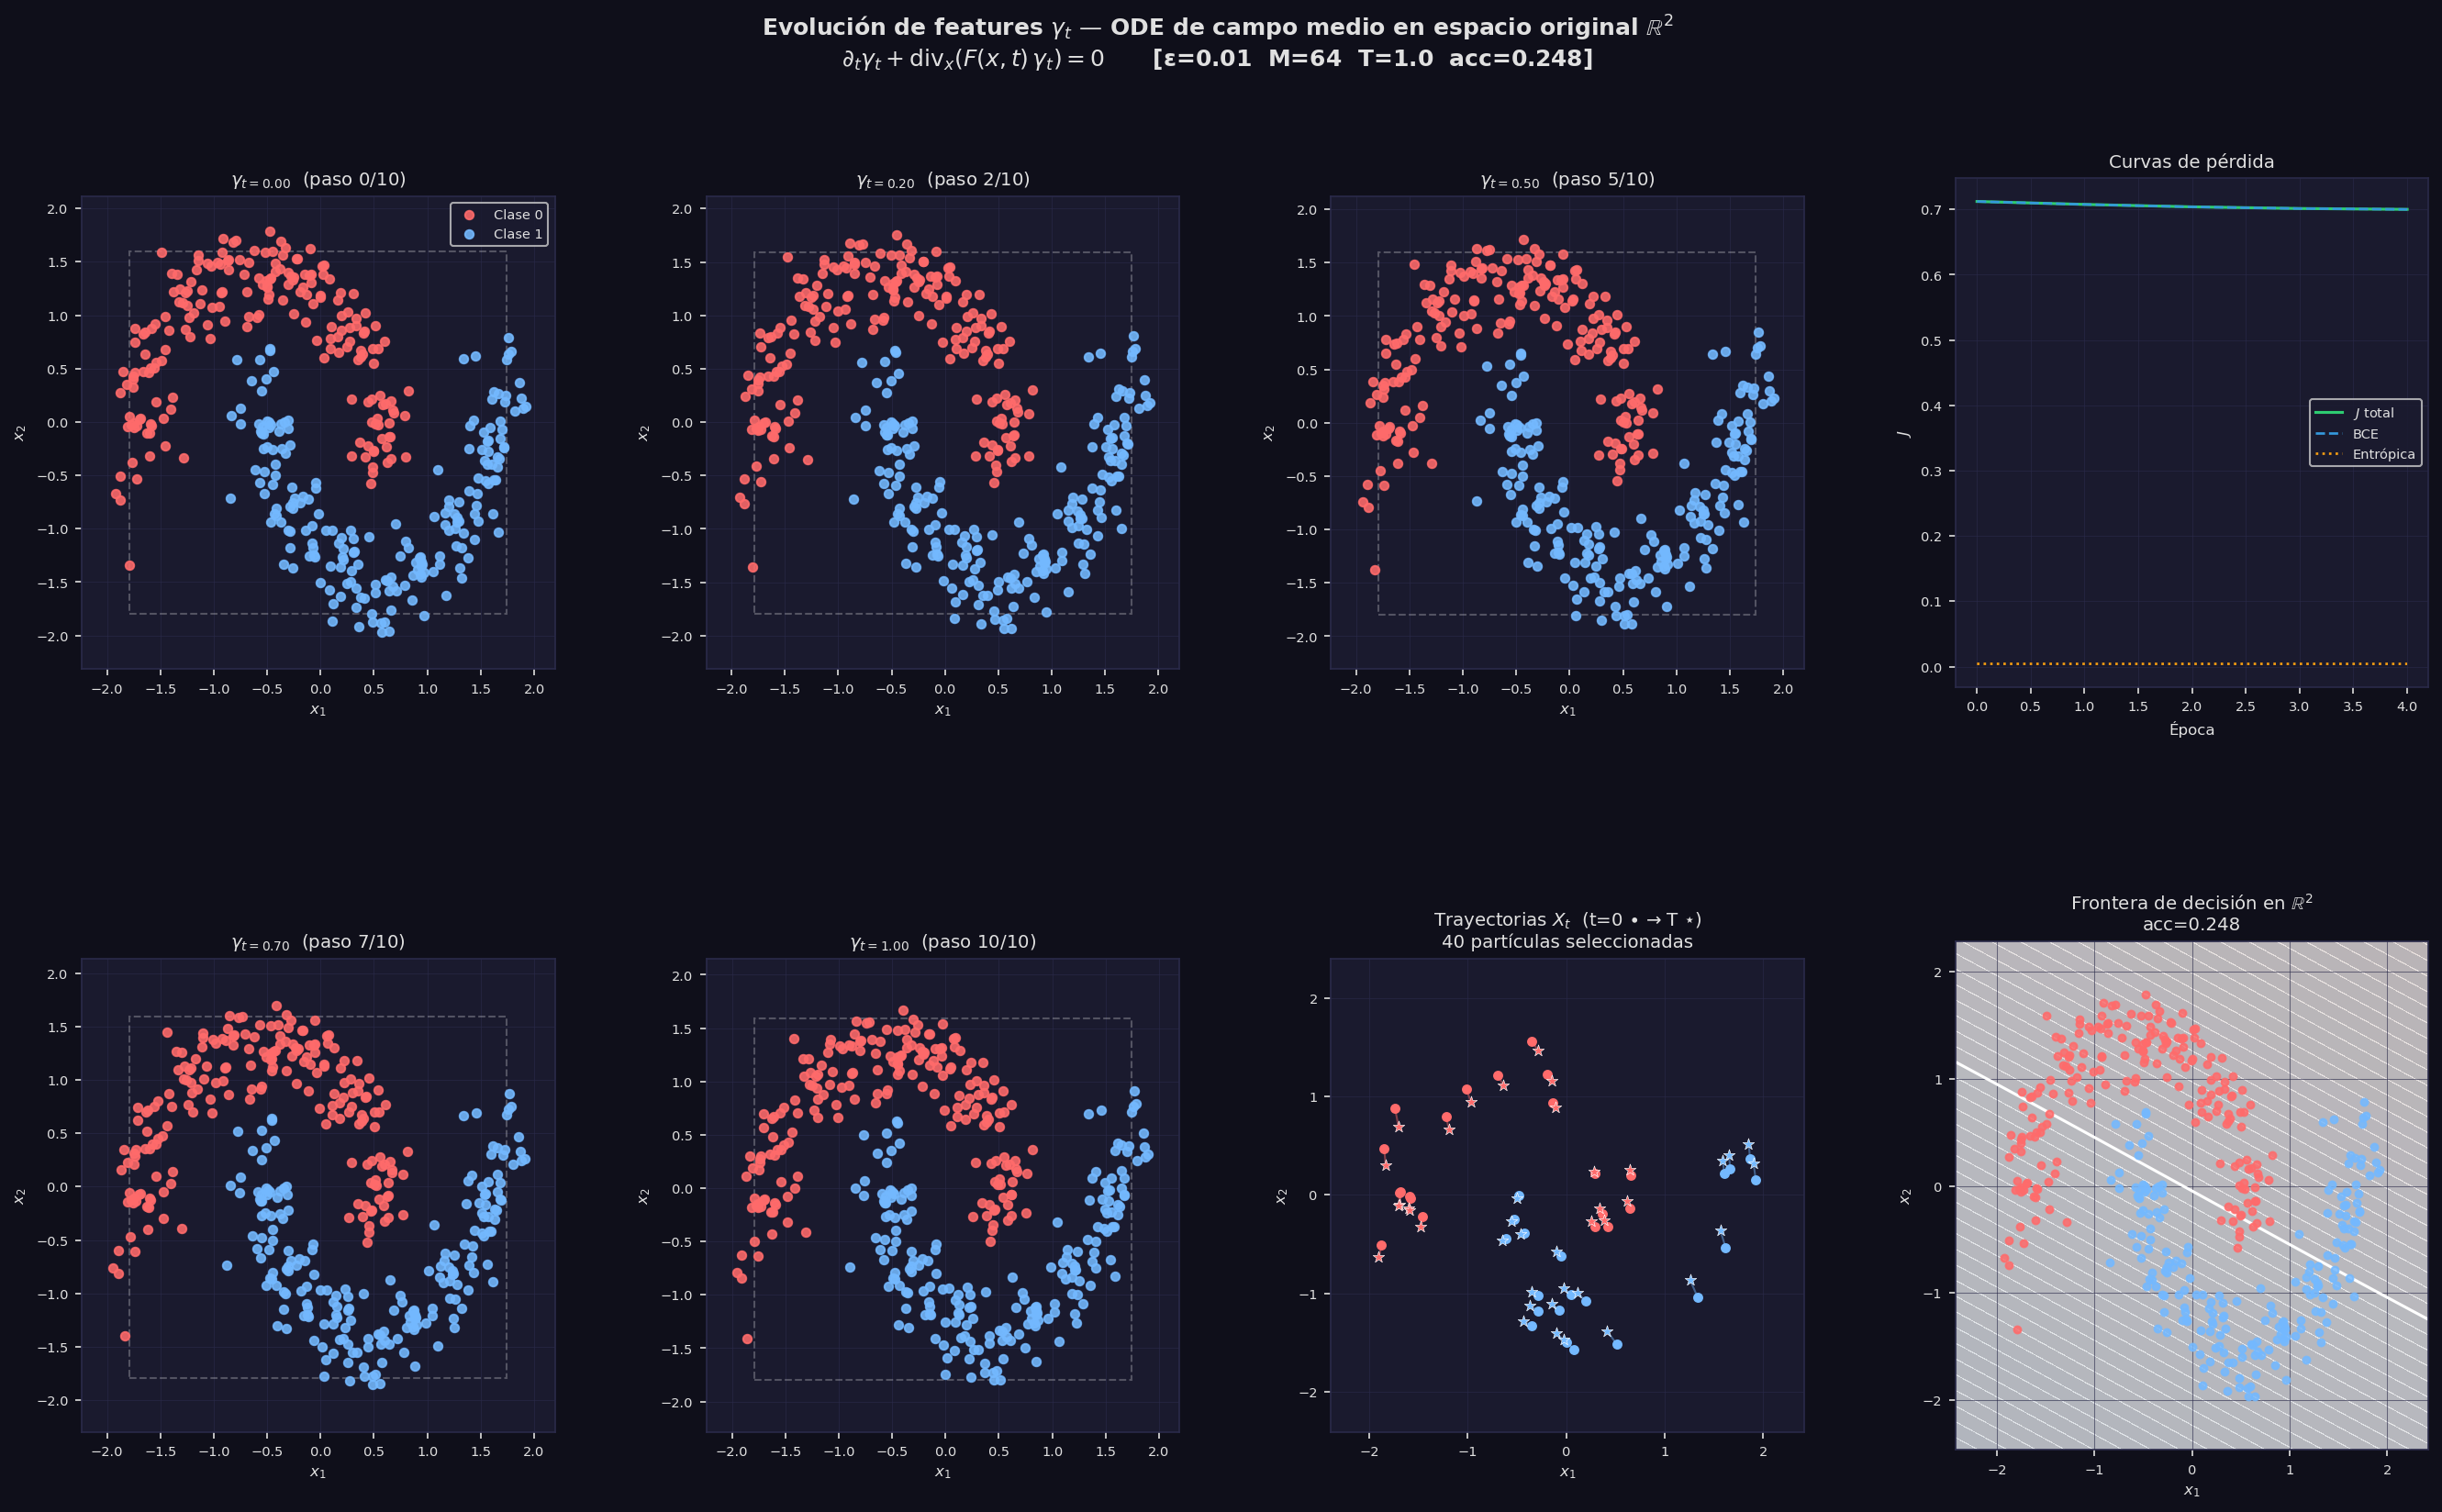
\includegraphics[width=0.92\linewidth]{../figuras/A_feature_evolution.png}
\end{center}

\end{frame}

% -------------------------------------------------------------------
\begin{frame}{Experimento A — Lectura de la figura}

\begin{columns}
\column{0.55\textwidth}
\begin{itemize}
  \item \textbf{Snapshots $\gamma_{t=0}\to\gamma_{t=T}$}: la marginal en $x$ de $\gamma_t$ coloreada según $Y_0^i$ (fija). Las lunas se deforman y separan progresivamente.
  \medskip
  \item \textbf{Trayectorias $X_t^i$}: 40 partículas (20 de cada clase) muestran que el campo $F(x,t)$ actúa de forma \textbf{colectiva} — característica del campo medio.
  \medskip
  \item \textbf{Frontera de decisión}: la isocurva $P(y=1|x) = 0.5$ en $\mathbb{R}^2$ es \textbf{altamente no lineal}, aunque el clasificador final $W\cdot X_T+b$ es lineal sobre $X_T$.
  \medskip
  \item \textbf{Accuracy final}: $100\%$.
\end{itemize}

\column{0.42\textwidth}
\begin{block}{Ecuación de continuidad}
\[
  \partial_t\gamma_t + \operatorname{div}_x(F\gamma_t)=0
\]
La «masa» se conserva y se transporta. El campo aprendido \textbf{hace que las clases se separen}, y el clasificador lineal explota esa separación.
\end{block}
\medskip
El rectángulo discontinuo en los snapshots indica la extensión original de $\gamma_0$: los puntos se han movido considerablemente respecto a la distribución inicial.
\end{columns}
\end{frame}

% ===================================================================
\section{Experimento B — Efecto de $\varepsilon$}

\begin{frame}{Experimento B — Curvas de convergencia (B1)}

\textbf{Objetivo:} estudiar el efecto de $\varepsilon\in\{0, 0.001, 0.01, 0.1, 0.5\}$ sobre la convergencia, las fronteras de decisión y la distribución de parámetros.

\begin{center}
  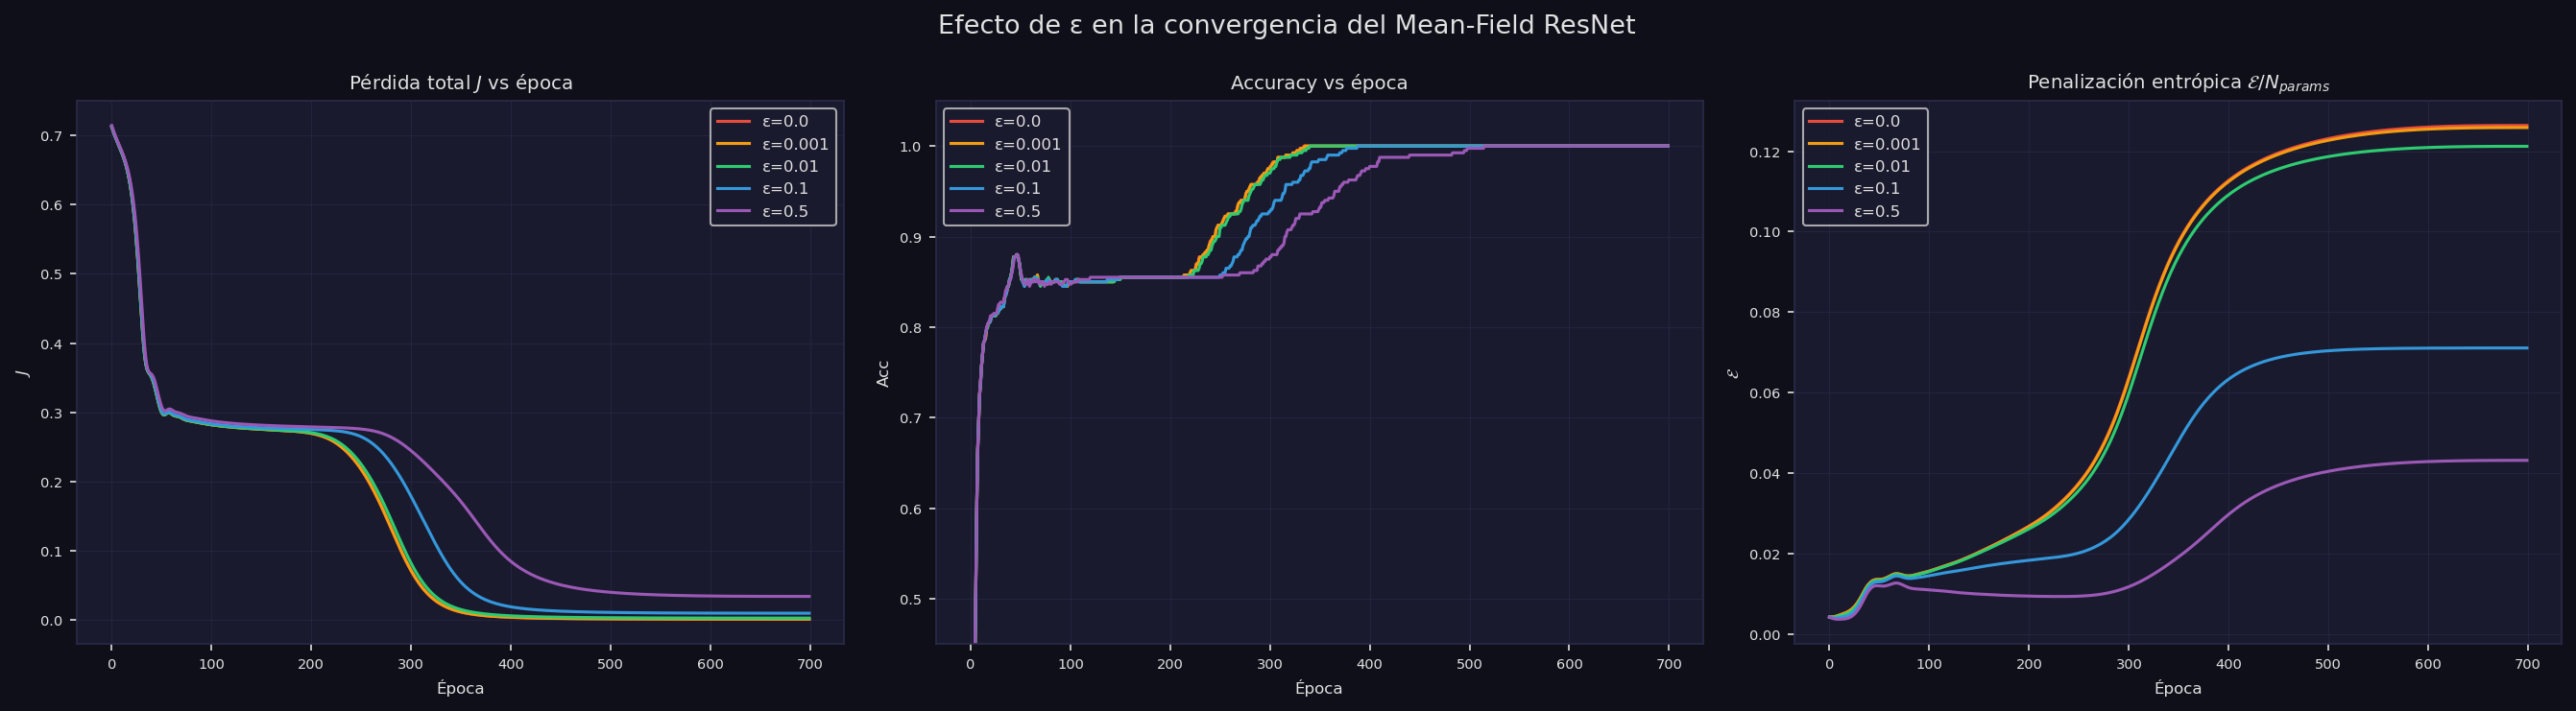
\includegraphics[width=0.90\linewidth]{../figuras/B1_convergence_curves.png}
\end{center}

\begin{columns}
\column{0.32\textwidth}
\textbf{Pérdida $J$:} mayor $\varepsilon$ $\Rightarrow$ mayor $J^*$ (más penalización). Velocidad comparable.
\column{0.32\textwidth}
\textbf{Accuracy:} todos alcanzan 100\%, incluyendo $\varepsilon=0.5$.
\column{0.32\textwidth}
\textbf{Penalización $\mathcal{E}$:} mayor $\varepsilon$ $\Rightarrow$ parámetros más cerca del prior $\nu^\infty$.
\end{columns}

\end{frame}

% -------------------------------------------------------------------
\begin{frame}{Experimento B — Fronteras de decisión (B2)}

\begin{center}
  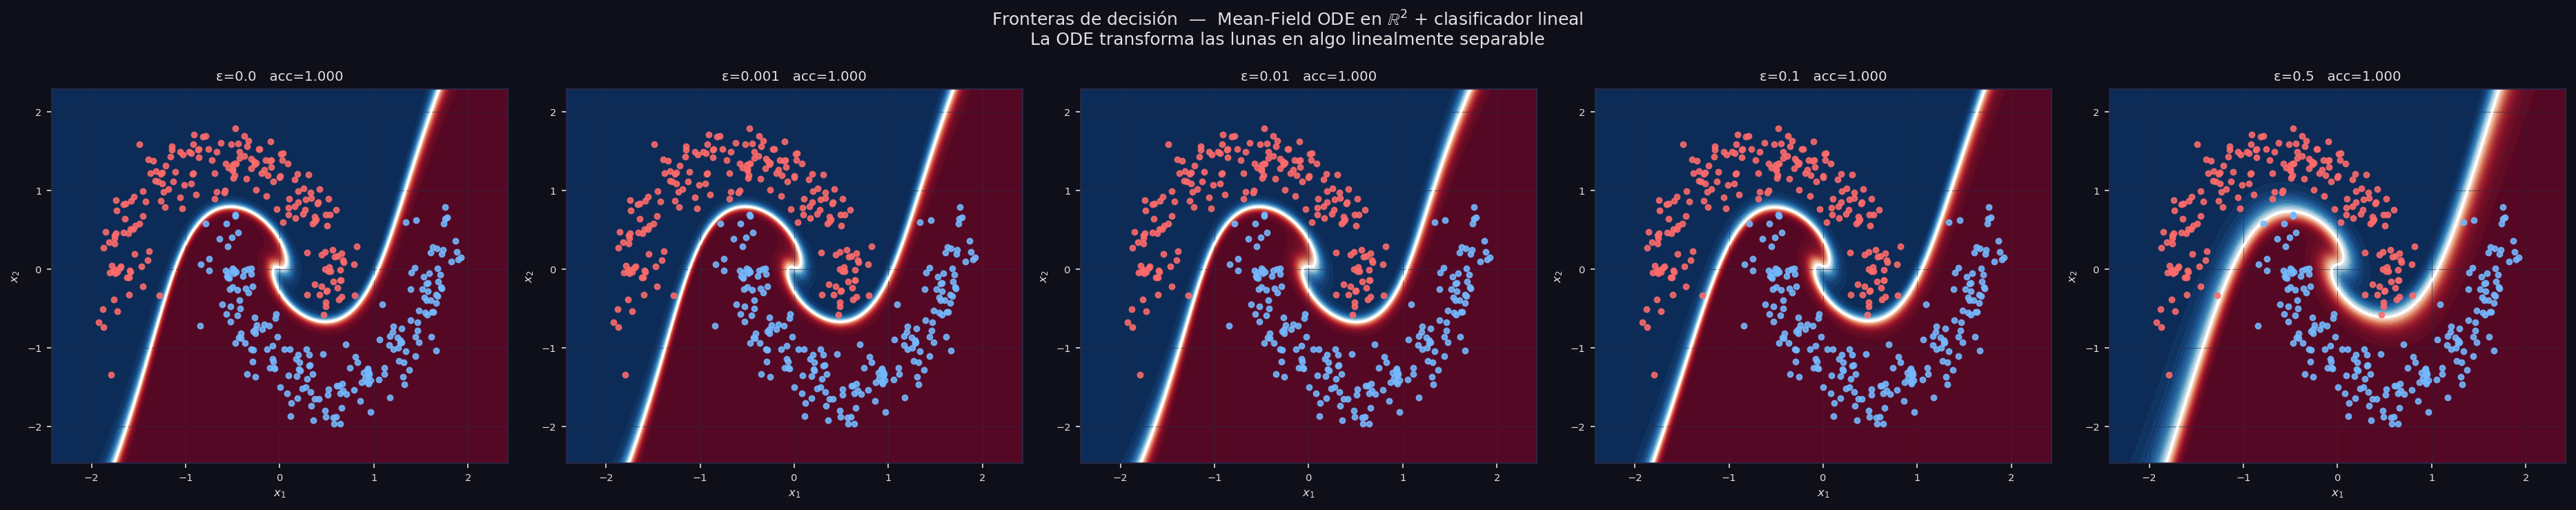
\includegraphics[width=0.92\linewidth]{../figuras/B2_decision_boundaries.png}
\end{center}

\begin{columns}
\column{0.50\textwidth}
El fondo muestra $P(y=1\mid x)$ en una malla 200×200: \textcolor{red}{rojo} $\approx P=0$, \textcolor{blue}{azul} $\approx P=1$, zona intermedia = incertidumbre.

La \textbf{línea blanca} es siempre la isocurva $P=0.5$ (frontera de clasificación).

\column{0.47\textwidth}
\begin{block}{Efecto de $\varepsilon$ en la frontera}
  Mayor $\varepsilon$ $\Rightarrow$ \textbf{zona de transición más ancha}: el modelo es menos seguro lejos de la frontera. $\varepsilon$ no solo suaviza la geometría sino que reduce la confianza del clasificador.
\end{block}
\end{columns}

\end{frame}

% -------------------------------------------------------------------
\begin{frame}{Experimento B — Prior de Gibbs: comportamiento MAP (B3)}

\begin{center}
  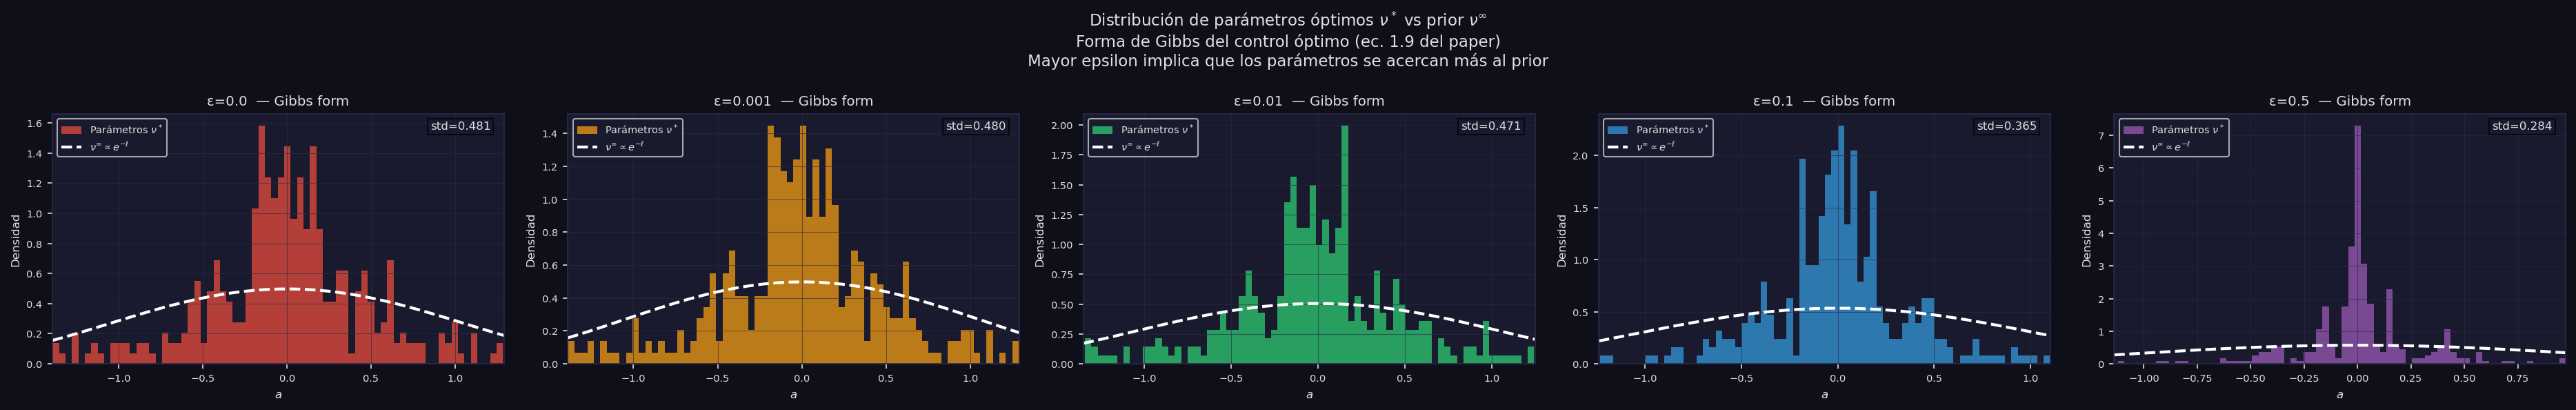
\includegraphics[width=0.72\linewidth]{../figuras/B3_gibbs_parameter_dist.png}
\end{center}

Los histogramas muestran la distribución empírica de $\sim 450$ parámetros al final del entrenamiento, comparada con el prior teórico $\nu^\infty\propto e^{-\ell(a)}$ (curva blanca discontinua).

\end{frame}

% -------------------------------------------------------------------
\begin{frame}{Experimento B — MAP y la forma de Gibbs}

\begin{columns}
\column{0.52\textwidth}
\begin{block}{¿Qué es MAP aquí?}
  Con parámetros deterministas + penalización L4+L2, minimizar $J$ equivale a \textbf{estimación MAP} bajo el prior $\nu^\infty$:
  \[
    \underbrace{-\log P(\text{datos}\mid\theta)}_{\text{BCE}} + \underbrace{\varepsilon\cdot\ell(\theta)}_{{-\log P(\theta)}} = J
  \]
  El resultado es un vector $\theta^*$ — no una distribución. El histograma muestra los $\sim 450$ valores MAP.
\end{block}

\column{0.44\textwidth}
\begin{block}{Desviación estándar vs.\ $\varepsilon$}
  \begin{tabular}{cc}
    \toprule
    $\varepsilon$ & $\mathrm{std}(\theta)$ \\
    \midrule
    0.0   & 0.481 \\
    0.001 & 0.480 \\
    0.01  & 0.471 \\
    0.1   & 0.365 \\
    0.5   & 0.284 \\
    \bottomrule
  \end{tabular}
  \medskip\\
  Mayor $\varepsilon$ $\Rightarrow$ parámetros más concentrados cerca del origen. Consistente con la forma de Gibbs.
\end{block}
\end{columns}

\bigskip
\begin{alertblock}{Cadena completa}
  $\text{Prior }\nu^\infty\;(\varepsilon\cdot\ell(\theta)\text{ en }J)\;+\;\text{Dataset }\gamma_0\;(\text{BCE})\;\xrightarrow{\text{Adam}}\;\theta^*_{\text{MAP}}$
\end{alertblock}

\end{frame}

% -------------------------------------------------------------------
\begin{frame}{Experimento B — Campo de velocidad (B4)}

\begin{center}
  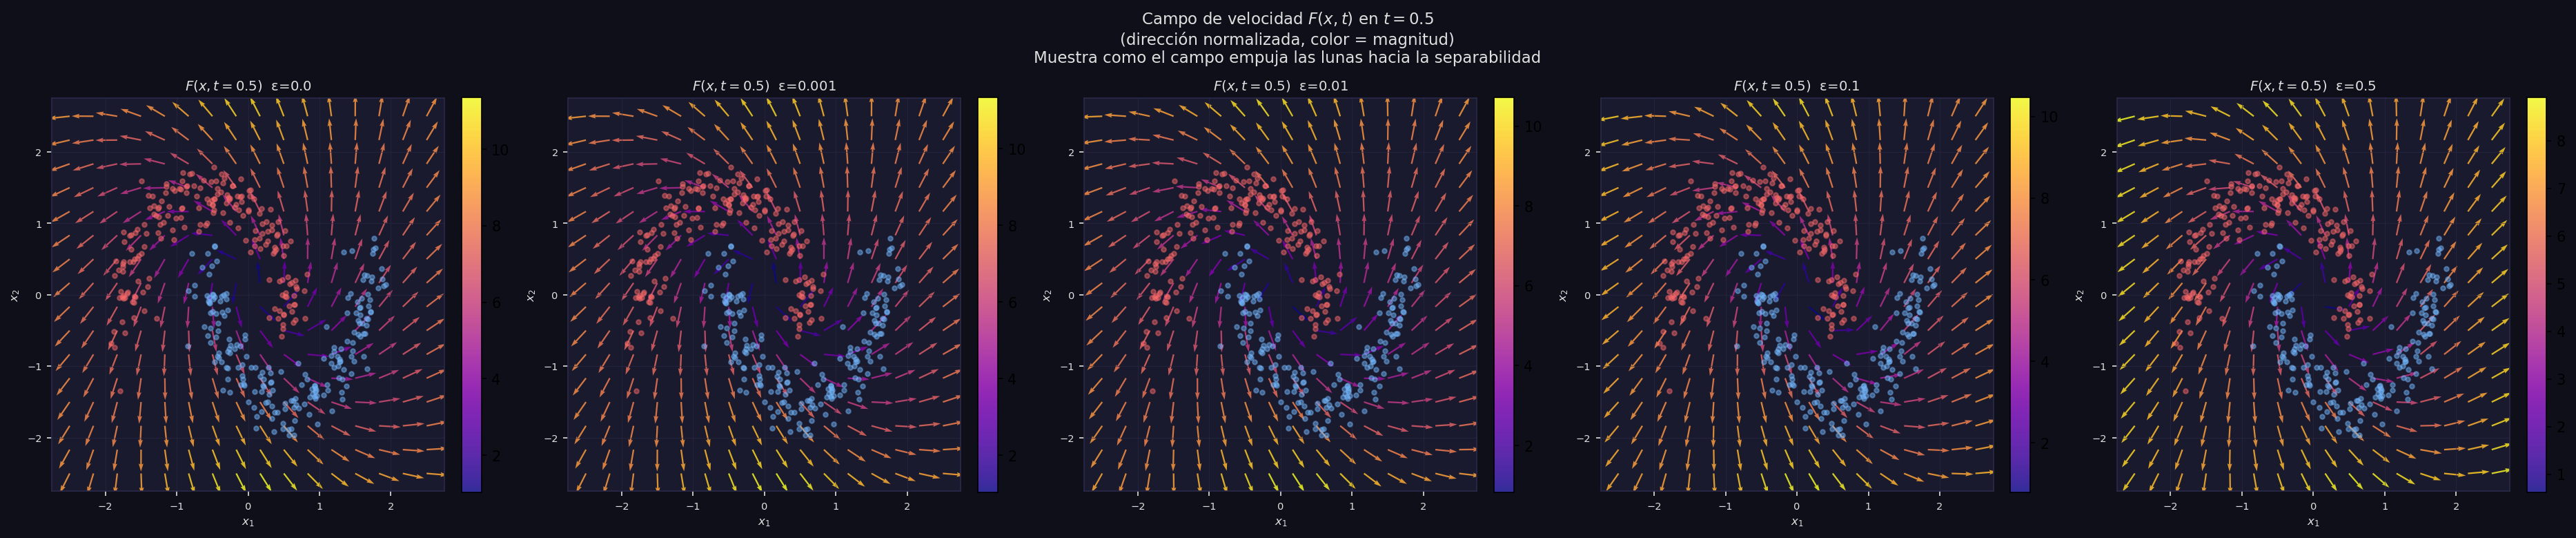
\includegraphics[width=0.85\linewidth]{../figuras/B4_velocity_field.png}
\end{center}

El campo $F(x,t=0.5)$ evaluado a mitad del flujo para cada $\varepsilon$. Las flechas muestran la dirección normalizada; el color indica la magnitud.

\medskip
El campo empuja los puntos de cada clase en direcciones distintas, creando la separación que el clasificador lineal explota. Mayor $\varepsilon$ produce campos más suaves.

\end{frame}

% ===================================================================
\section{Experimento C — Verificación de la condición PL}

\begin{frame}{Experimento C — Verificación empírica de la condición PL}

\textbf{Objetivo:} comprobar que $\|\nabla J(\theta)\|^2 \geq 2\mu(J(\theta)-J^*)$ se cumple empíricamente durante el entrenamiento (Meta-Teorema 2).

\begin{center}
  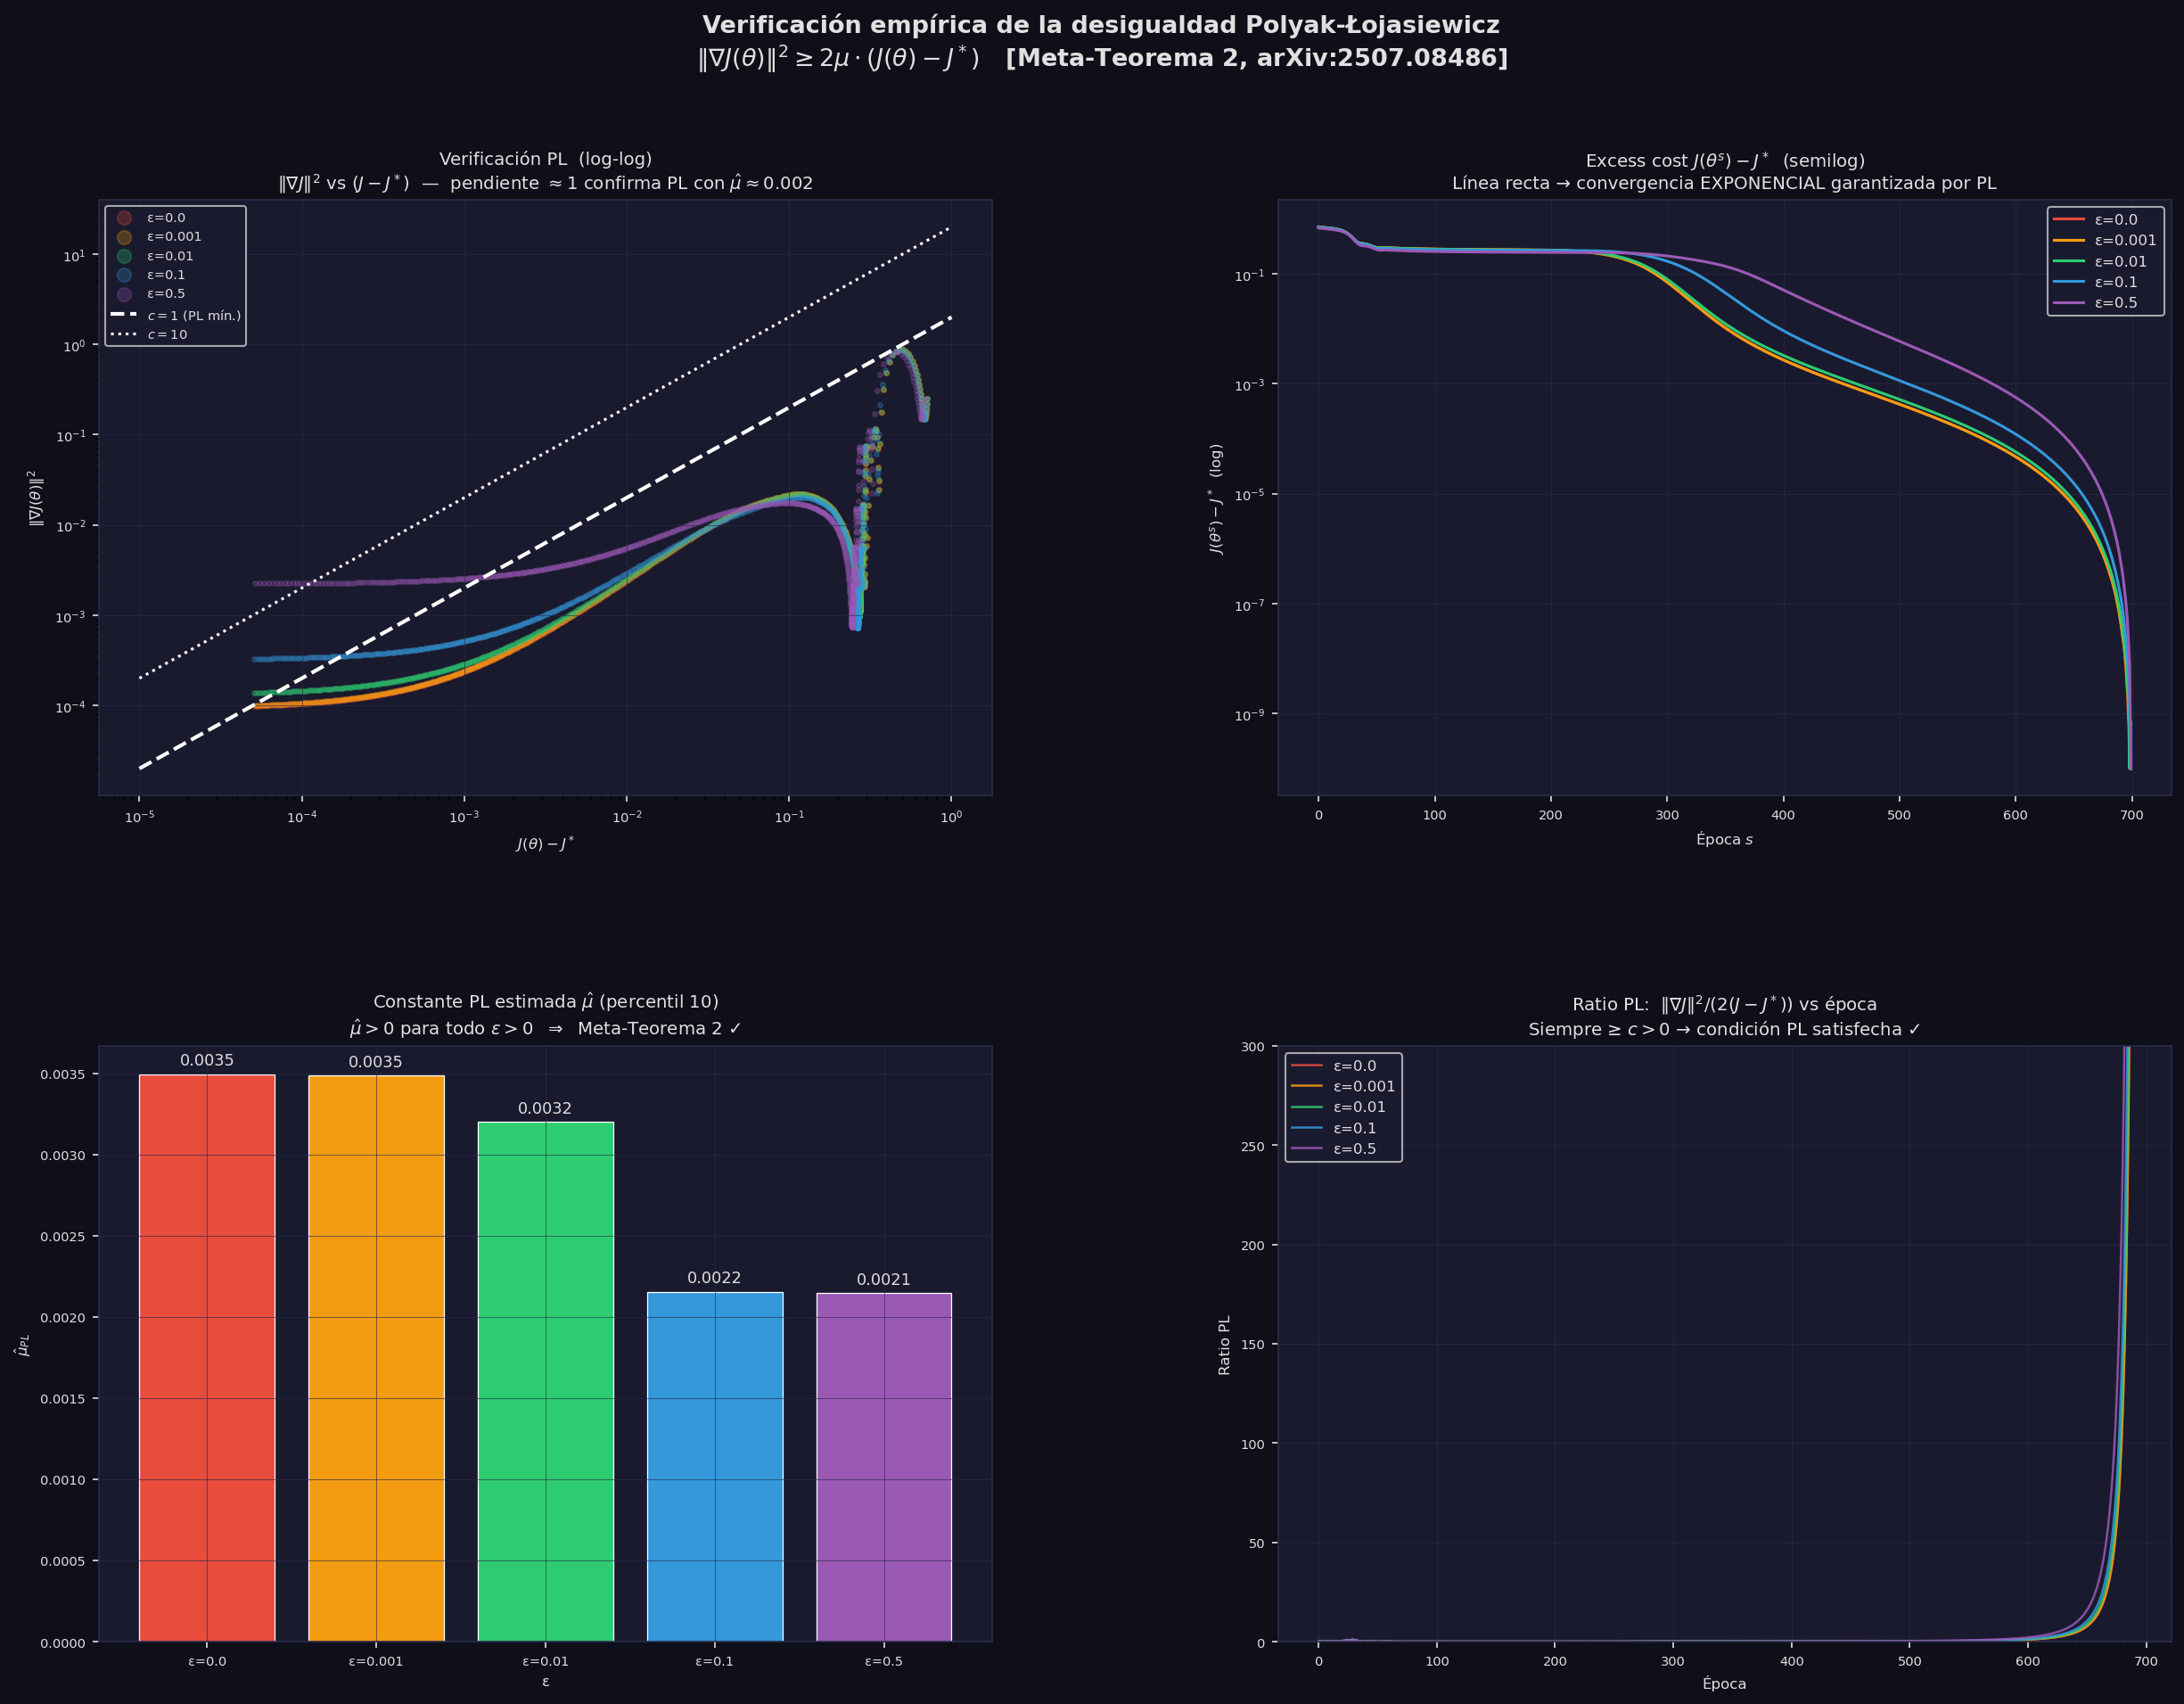
\includegraphics[width=0.88\linewidth]{../figuras/C_pl_verification.png}
\end{center}

\end{frame}

% -------------------------------------------------------------------
\begin{frame}{Experimento C — Lectura de los paneles}

\begin{columns}
\column{0.48\textwidth}
\textbf{C1 — Diagrama log-log:}\\
Cada punto = una época. Eje X: $J-J^*$; eje Y: $\|\nabla J\|^2$.

La nube sigue una tendencia con \textbf{pendiente $\approx 1$} en log-log: firma visual de la condición PL.

Las rectas blancas son referencias para $c=1$ y $c=10$; los puntos están por debajo porque $\hat\mu\approx 0.002\ll 1$ (la condición solo exige $\mu>0$).

\bigskip
\textbf{C2 — Semilog:}\\
Curvas aproximadamente lineales $\Rightarrow$ decay \textbf{exponencial}:
\[
  J(\theta_s)-J^* \lesssim (J_0-J^*)\,e^{-2\mu s}
\]

\column{0.48\textwidth}
\begin{block}{C3 — Constante $\hat\mu_{PL}$ por $\varepsilon$}
  \begin{tabular}{cc}
    \toprule
    $\varepsilon$ & $\hat\mu_{PL}$ \\
    \midrule
    0.0   & 0.0035 \\
    0.001 & 0.0035 \\
    0.01  & 0.0032 \\
    0.1   & 0.0022 \\
    0.5   & 0.0021 \\
    \bottomrule
  \end{tabular}
\end{block}

\begin{alertblock}{Resultado clave}
  $\hat\mu > 0$ para \textbf{todos} los $\varepsilon$. La condición PL se cumple incluyendo el régimen sin garantía teórica ($\varepsilon=0$).
\end{alertblock}

\medskip
\textbf{C4:} el ratio $\|\nabla J\|^2/(2(J-J^*))$ permanece $>0$ durante \textbf{todas} las épocas, incluyendo el final del entrenamiento.
\end{columns}

\end{frame}

% ===================================================================
\section{Conclusiones}

\begin{frame}{Conclusiones}

\begin{block}{Evidencia empírica de los resultados teóricos de Daudin \& Delarue (2025)}
\begin{tabular}{p{0.44\linewidth}p{0.50\linewidth}}
  \toprule
  Resultado del paper & Verificación empírica \\
  \midrule
  La ODE transforma $\gamma_0$ en $\gamma_T$ separable &
    Exp.\ A: lunas $\to$ puntos separados, acc $= 100\%$ \\[4pt]
  $\varepsilon>0$ concentra el control cerca de $\nu^\infty$ &
    Exp.\ B3: std$(\theta)$ decrece con $\varepsilon$ — MAP consistente con la predicción de Gibbs \\[4pt]
  Condición PL: $\|\nabla J\|^2\geq 2\mu(J-J^*)$, $\mu>0$ &
    Exp.\ C: ratio PL $>0$ en todas las épocas, $\hat\mu\approx 0.002$ \\[4pt]
  Convergencia exponencial bajo PL &
    Exp.\ C2: decay lineal en escala log \\
  \bottomrule
\end{tabular}
\end{block}

\bigskip
\begin{columns}
\column{0.48\textwidth}
\begin{alertblock}{Aproximaciones implementadas}
  \begin{itemize}
    \item Augmentación temporal (restringe $\nu_t$)
    \item Solo término de energía en KL (sin entropía)
    \item Muestras finitas de $\gamma_0$
  \end{itemize}
\end{alertblock}
\column{0.48\textwidth}
\begin{block}{Posibles extensiones}
  \begin{itemize}
    \item Scaling de $\hat\mu$ con $M$, $d_1$, $\varepsilon$
    \item Comparación con redes sin campo medio
    \item Análisis del error de discretización RK4
  \end{itemize}
\end{block}
\end{columns}

\end{frame}

% -------------------------------------------------------------------
\begin{frame}{Referencias}

\begin{thebibliography}{9}
\bibitem{daudin2025}
  Daudin, S.\ \& Delarue, F.\ (2025).
  \textit{Genericity of the Polyak-Łojasiewicz inequality for mean-field Neural ODEs with entropic regularization.}
  arXiv:2507.08486.

\bibitem{chen2018}
  Chen, R.T.Q., Rubanova, Y., Bettencourt, J.\ \& Duvenaud, D.\ (2018).
  \textit{Neural Ordinary Differential Equations.}
  NeurIPS 2018.

\bibitem{carmona2018}
  Carmona, R.\ \& Delarue, F.\ (2018).
  \textit{Probabilistic Theory of Mean Field Games with Applications.}
  Springer.

\bibitem{polyak1963}
  Polyak, B.T.\ (1963).
  \textit{Gradient methods for the minimisation of functionals.}
  USSR Computational Mathematics and Mathematical Physics, 3(4), 864--878.
\end{thebibliography}

\end{frame}

% -------------------------------------------------------------------
\begin{frame}{}
  \begin{center}
    \Large\textbf{Gracias}\\[1em]
    \normalsize
    Código disponible en:\\
    \texttt{daudin\_delarue\_moons.py}\\[1em]
    Beca JAE Intro — CSIC\\
    Tutor: Rafael Orive
  \end{center}
\end{frame}

\end{document}
